\documentclass[10pt]{article}

\usepackage{float}
\usepackage[T1]{fontenc}
\usepackage[utf8]{inputenc}
\usepackage[english]{babel}
\usepackage{amssymb,amsfonts,amsmath,amsthm}
\usepackage{graphicx}
\usepackage{lmodern}
\usepackage{mdframed}
\usepackage{hyperref}
\usepackage{cases}
\usepackage{framed}
\usepackage{pdfpages}
\usepackage{multicol}
\usepackage[margin=60pt]{geometry}
\usepackage{abstract}
\renewcommand{\abstractnamefont}{\normalfont\Large\bfseries}
\renewcommand{\abstracttextfont}{\normalfont\normalsize}

\usepackage{pgfplots}
%\usepgfplotslibrary{colormaps}
\pgfplotsset{every axis/.append style={line width=1pt}}

\usepackage{adjustbox}
\newcommand{\specialcell}[2][c]{%
	\begin{tabular}[#1]{@{}c@{}}#2\end{tabular}}

\newcommand{\avg}[1]{\left< #1 \right>} % for average
\newcommand{\Ne}{N_\mathrm{e}}

\begin{document}
\includepdf[pages={1}]{frontpage.pdf}
	\begin{abstract}
		Adaptation in protein-coding sequences can be detected, and quantified, using two different types of methods: using either multiple sequence alignment across species (and phylogenetic codon models), or by combining divergence and polymorphism data (McDonald-Kreitman tests).
		Phylogenetic codon models are classically formulated in terms of the relative synonymous and non-synonymous substitution rates. However, because of the background of purifying selection, these models are limited in their sensitivity.	
		Recent developments, conducted in the host lab, have led to more sophisticated mechanistic codon models aiming at making a more detailed quantitative assessment of the interplay between mutation, purifying and positive selection, leading to potentially more powerful detection of adaptation.
		These models however, have not yet been tested on a broad scale.
		Similarly, McDonald-Kreitman tests can be sensitive to the exact interplay between adaption and purifying selection, and more elaborate version of these tests, using models derived from population genetic theory, have been developed over the last years.
		The aim of this project is to conduct a large scale analysis on mammalian protein-coding sequences, using a combination of inter- and intra-specific data across the entire exome.
		A detailed comparison between the two types of approaches will be conducted, using classical and mechanistic codon models, as well as MK tests.
		This will allow for a general assessment of the congruence between these methods, and will also give a broad-scale picture of the patterns of adaptation in mammalian exomes.
		
		
		\smallskip
		\noindent \textbf{Keywords.} Evolution, Adaptation, Coding Sequences, Codon models, Synonymous/Non-synonymous substitution.
	\end{abstract}
	\begin{multicols}{2}
	\section*{Introduction}

	Molecular sequences are shaped over time by different evolutionary forces such as mutation, selection and random drift \cite{ohta_nearly_1992}. Selection takes a variety of forms since a mutation in a molecular sequence can either be neutral, positively or negatively selected. More globally, different proteins might be in different selection regimes. Some, mostly under strong purifying selection, are expected to be stable trough time.
	Other proteins, involved in a arm race as for example against pathogens, are under recurrent positive selection and tend to evolve faster \cite{enard_viruses_2016}. One main goal of molecular evolution is to quantify the intensity of evolutionary forces acting on sequences, and to detect the signature in present-day sequences left by recurrent events of positive selection. \\
	
	Theoretically, in order to detect positive selection, one must have data where part of the sequence is known to be under a neutral regime, which can be used as a null model. In the case of protein-coding DNA sequences, a mutation will either be synonymous (not changing the translated amino-acid), or non-synonymous (such that the translated amino-acid will be different). Synonymous sites are usually taken as proxies for neutral sites, although they may be under weak selection. Non-synonymous mutations, on the other hand, are under a mixture of adaptation, purifying selection and random drift, depending on the selection coefficient associated with the new amino-acid. The synonymous sites are used to quantify the neutral process, and the deviation to this neutral process on non-synonymous sites gives insight on the strength of both positive and purifying selection. \\
	
	Contrasting synonymous and non-synonymous changes, two different types of methods have emerged to quantify both positive and purifying selection acting on protein-coding sequences.
	One method, stemming from population genetics, contrasts polymorphism inside a population and divergence to a close species. In the following, this method will be called population-based inference. Another method, stemming from phylogeny, uses multiple sequence alignment in different species to quantify adaptation. This method will be called phylogeny-based inference. One goal of the present work is to confound these two types of approaches.\\
	
	In population-based inference, one of the most widely used test for adaptation was proposed by McDonald and Kreitman \cite{McDonald1991}. This method uses the substitutions (mutations that reach fixation) between two close species and polymorphism (sites with at least two alleles) inside on population. Under a neutral regime, deleterious mutations are assumed to occur, but are quickly removed by selection, and the ratio of non-synonymous substitutions over synonymous substitutions ($d_N/d_S$) is expected to be lower than one, since none of non-synonymous deleterious mutations will reach fixation. Also the ratio of non-synonymous polymorphism over synonymous polymorphism ($p_N/p_S$) is also expected to be lower than one, since the non-synonymous deleterious mutations will be removed quickly from the population. Most importantly, in the absence of advantageous mutations, these two ratio are expected to be the same ($d_N/d_S=p_N/p_S$). If advantageous mutations occur, then they are fixed rapidly in the population, thus contributing solely to divergence but not to polymorphism, leading to an overall $d_N/d_S$ greater than $p_N/p_S$ \cite{smith_adaptive_2002, kimura_neutral_1983}. In the end, the method can therefore leads to a decomposition in the total rate rate of evolution ($d_N/d_S$) into two components: respectively neutral ($p_N/p_S$) and adaptive ($d_N/d_S-p_N/p_S$). This method is however plagued by the presence of moderately deleterious non-synonymous mutations, which can segregate at substantial frequency in the population without reaching fixation, thus contributing solely to polymorphism, and not to divergence, potentially resulting on an under-estimation of the rate of adaptive evolution \cite{eyre-walker_quantifying_2002}. Subsequent developments have tried to correct for this effect be relying on an explicit \textit{nearly-neutral model}, so as to derive the expected value of $d_N/d_S$ and $p_N/p_S$ in the absence of adaptation, the observed deviation of $d_N/d_S$ compared to this null expectation then provides estimates of the rate of adaptation \cite{eyre-walker_estimating_2009, galtier_adaptive_2016}.
	
	Phylogeny-based inference models the substitution rate at the codon level. Synonymous and non-synonymous mutations are treated differently. The rate of non-synonymous substitutions over the rate of synonymous substitutions (denoted $\omega=d_N/d_S$) is estimated as a parameter of the model \cite{Muse1994,Goldman1994}. Assuming synonymous mutations are neutral, an $\omega>1$ signals an excess in the rate of non-synonymous substitutions, indicating that the protein is under adaptive evolution. Conversely, a default of non-synonymous substitutions, leading to $\omega<1$, means the protein is under purifying selection. However, in practice, protein are typically under a mix of adaptation and purifying selection, thus typically leading to an $\omega<1$ even in the presence of positive selection. More sophisticated methods have been proposed. In particular, site-model trying to detect specific site of the sequence with an $\omega>1$, has been applied \cite{Yang2001, kosiol_patterns_2008}. However they potentially misses a substantial fraction of adaptation and does not quantify the rate of adaptation. An alternative approach to phylogenetic codon models would be to do as in the case of population-based inference mentioned above, to rely on an explicit \textit{nearly-neutral model} as the null model against which to detect deviation of $\omega=d_N/d_S$. In this direction, mutation-selection models provides a null model by estimating fitness of amino-acids \cite{Yang2008, Halpern1998, Rodrigue2010}. By modeling the fitness landscape of amino-acids, at equilibrium the codons will bounce between amino-acids with high fitnesses, and mutation from a high fitness amino-acid towards a low fitness amino-acid will have a small probability of fixation, and the model genuinely takes into account purifying selection. By contrasting $\omega$ estimated by the classical codon models and the $\omega$ predicted by the mutation-selection model, one can hope to extract the rate of adaption, but this has not yet been conducted on a large scale \cite{Rodrigue2016}.
	
	Using protein-coding sequences, 
	Although population- and phylogeny-based inference both estimate the rate of adaptation, the congruence between the two methods has not yet been asserted. In this study, we analyzed 1355 protein-coding (CDS) orthologs in mammals, and conducted two separate analysis on these CDS. First, alignments in mammals (except \textit{Homo sapiens} and \textit{Pan troglodytes}) were used to run site-model and mutation-selection site-model. We estimated the rate of adaptation in each CDS, and extracted CDS with a rate of adaptation significantly high. Secondly, population-based inference was conducted using polymorphism available in \textit{Homo sapiens} and divergence to \textit{Pan troglodytes}. We tested if the group of sequences detected with a high rate of adaption in the phylogeny-based inference also display a high rate of adaptation in population-based inference.

	\section*{Materials and methods}
	\begin{figure*}[ht!]
	\begin{mdframed}
		\centering
		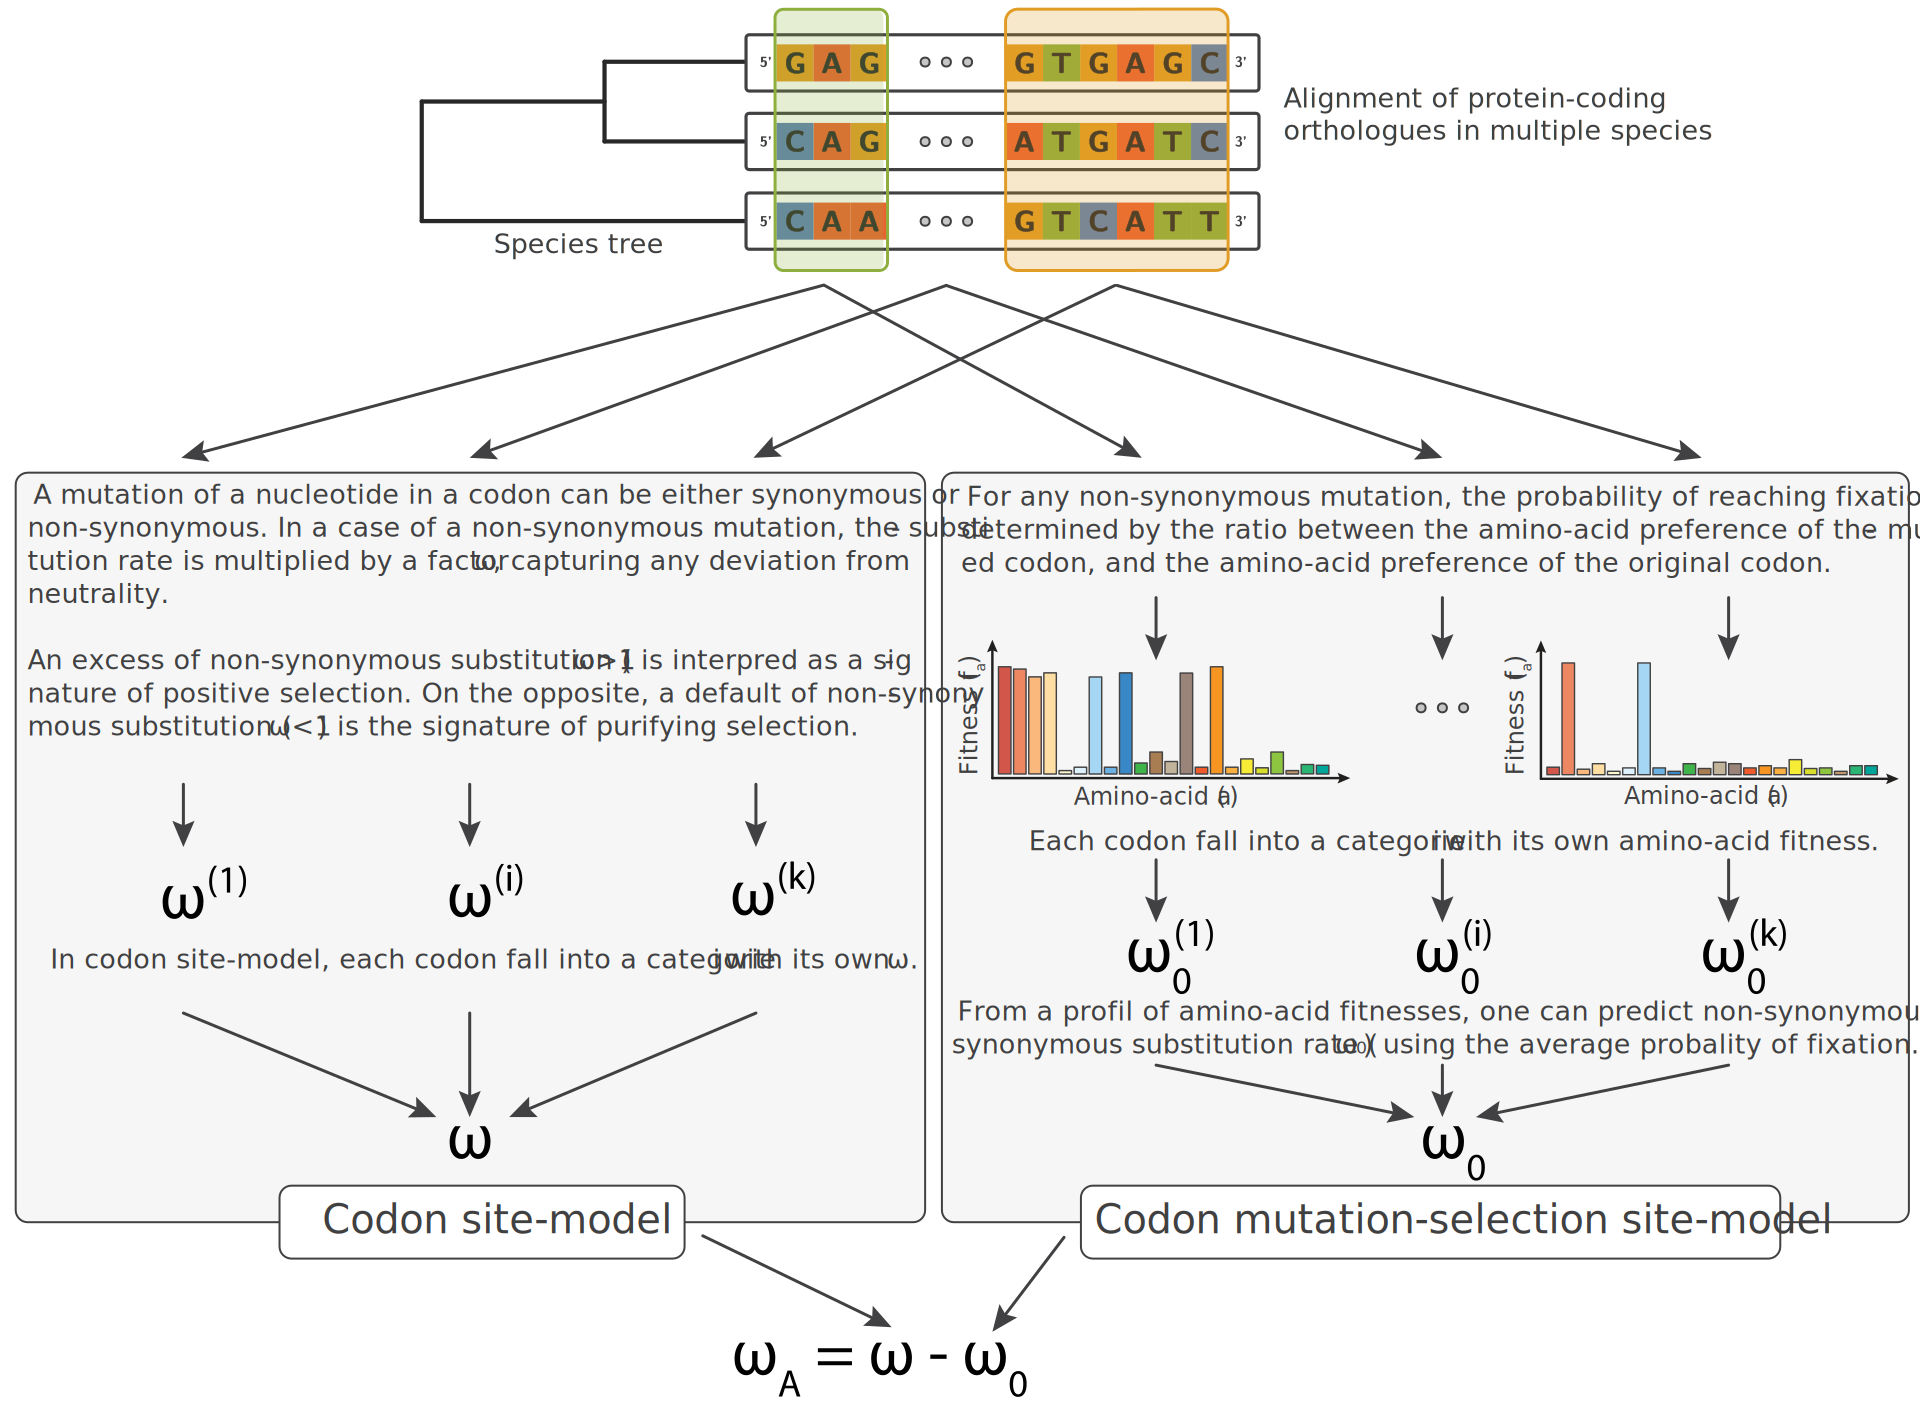
\includegraphics[width=\textwidth]{../Figures/codon_model.pdf}\\
		\caption{ \textbf{Phylogeny-based inference of $\omega_A$}. On the left panel, codon site-model estimates $\omega$ as the average of $\omega^{(i)}$. On the right panel, mutation-selection (mut-sel) model estimates the fitness of each amino-acid on each site. From the profile of amino-acid, one can compute $\omega_{0}$ which is the predicted rate of non-synonymous over synonymous substitution at the mutation-selection balance and genuinely taking into account purifying selection. Both methods runs independently from the same alignment data. From these two independent runs,  $\omega_A$ is computed as the difference $\omega - \omega_{0}$\label{fig:codon_model}}
	\end{mdframed}
	\end{figure*}
	\subsection*{Rate of adaption in phylogeny-based inference }
	Codon models estimate a single parameter $\omega$, namely the ratio of the non-synonymous over the synonymous substitution rates, capturing any deviation from neutrality over the entire sequence and along all branches of the phylogenetic tree \cite{Muse1994,Goldman1994}. In codon site-models, the codons are separated into a finite number of different categories, with each category $i$ having its own $\omega^{(i)}$ \cite{Yang2001}. More flexible, in infinite mixture models, the number of categories is not fixed in advance and is estimated during the computation. More specifically, $\omega^{(i)}$ are drawn from an infinite mixture using a Dirichlet process \cite{Huelsenbeck2006}. In codon site-models, the global $\omega$ is computed as the average of the $\omega^{(i)}$ (see figure \ref{fig:codon_model}, left panel). 
	
	In mutation-selection site-models \cite{Yang2008, Halpern1998, Rodrigue2010}, the rate of non-synonymous substitution from codon $a$ to codon $b$ ($q_{a \mapsto b}$) is equal to the rate of mutation ($\mu$) multiplied by the probability of fixation of the mutation ($p_{a \mapsto b}$) \cite{kimura_neutral_1983}. Crucially, the probability of fixation depends on the difference of fitness between the amino-acid encoded by the mutated codon ($f_b$) and the fitness of the amino-acid encoded by the original codon ($f_a$) \cite{wright_evolution_1931, fisher_genetical_1930}. Altogether, the rate of substitution from codon $a$ to $b$ is:
	\begin{equation*}
		q_{a \mapsto b} = \mu \dfrac{\mathrm{ln}(f_b / f_a)}{1 - f_b / f_a}.
	\end{equation*}
	
	Once the amino-acid fitness are estimated, one can compute $\omega_{0}$, the predicted rate of non-synonymous over synonymous substitution at the mutation-selection balance (see figure \ref{fig:codon_model}, right panel): 
	\begin{align*}
	\omega_{0} &= \sum_a \dfrac{1}{61} \sum_b \dfrac{1}{61} q_{a \mapsto b} \\ &= \mu \sum_a \dfrac{1}{61} \sum_b \dfrac{1}{61} \dfrac{\mathrm{ln}(f_b / f_a)}{1 - f_b / f_a}, 
	\end{align*}
	where $a$ and $b$ are all the possible codons ($61$ by discarding stop codons) \cite{Spielman2015}.
	Under the assumption that the fitness profile is stable in time, then the predicted $\omega_0$ (mutation-selection site-model) and the estimated $\omega$ (site-model) should be the same. But if the assumption that fitness landscape are stable in time is broken, then $\omega > \omega_0$ since the predicted $\omega_{0}$ at the mutation-selection balance is always over-estimating the fitness of current the amino-acid and the codon will stay longer on the current amino-acid than it should, thus under-estimating the probability of fixation of non-synonymous mutations.
	From these consideration, we estimate $\omega_A$, namely the rate of adaptive substitution over neutral substitution as the deviation of $\omega$ from the quasi-neutral model $\omega_0$ (see figure \ref{fig:codon_model}):
	\begin{equation*}
		\omega_A = \omega - \omega_0.
	\end{equation*}
	
	With this protocol, a two steps procedure is needed and one needs to run independently site-model and mutation-selection site-model. It has also been suggested to run the mutation-selection model with one additional global parameter ($\omega^*$) \cite{Rodrigue2016}. It this model, each non-substitution mutation has a probability of fixation determined by amino-acid fitness profile, but overall multiplied by the parameter $\omega^*$. In a one run,  $\omega_0$ is estimated as well as $\omega^*$, which capture deviation from the mutation-selection model. The rate of adaptive evolution is:
	\begin{equation}
		\omega_A^* = \omega_0 (\omega^* - 1 ).
	\end{equation}
	
			\begin{figure*}[hb!]
			\begin{mdframed}
				\centering
				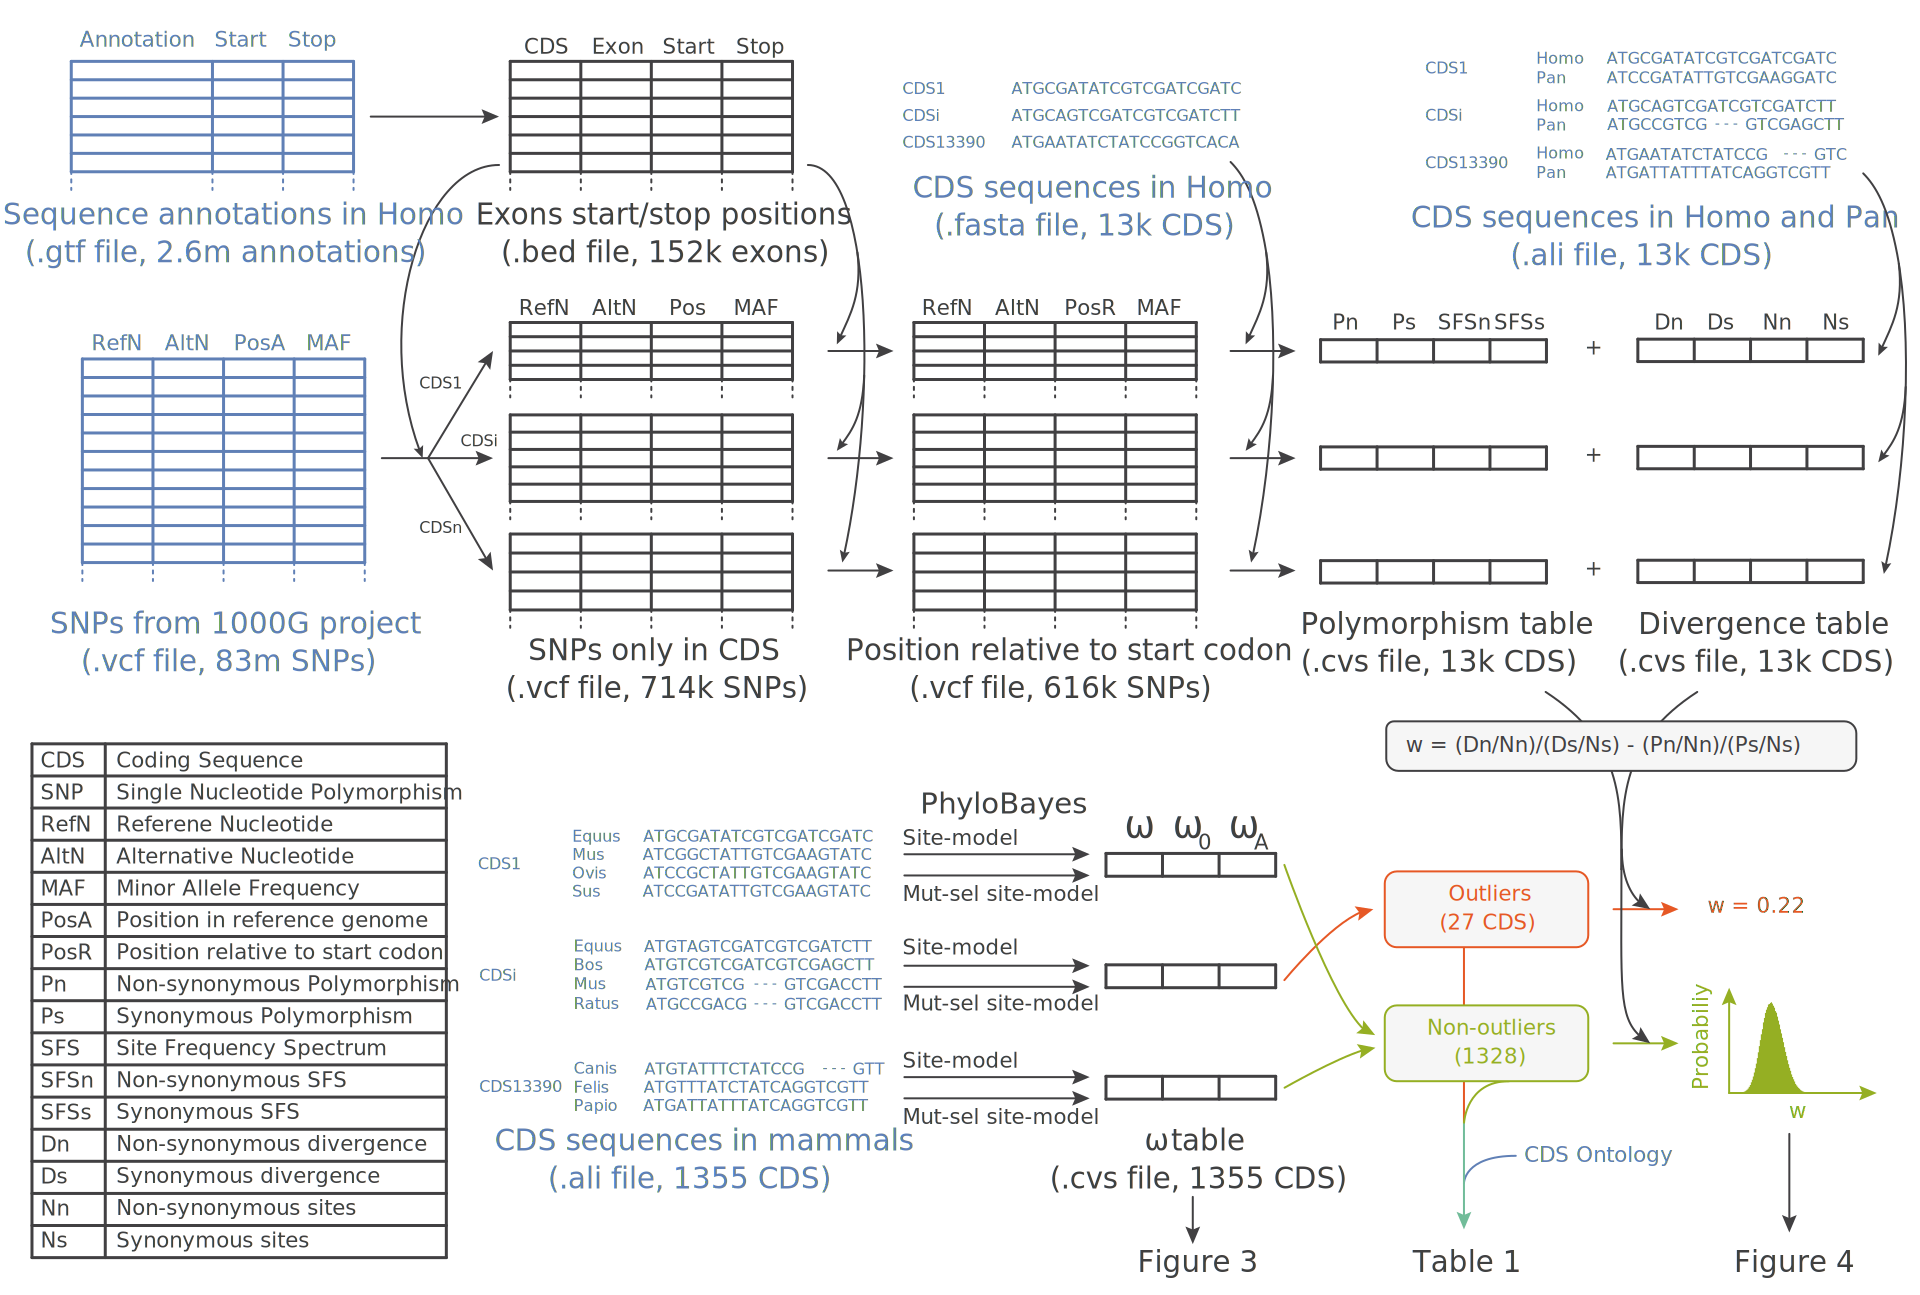
\includegraphics[width=\textwidth]{../Figures/pipeline.pdf}\\
				\caption{ \textbf{The pipeline for data analysis}. In blue are the input data necessary to run the analysis. In black solid arrows are python custom scripts.  \label{fig:pipeline}}
			\end{mdframed}
		\end{figure*}
	\subsection*{PhyloBayesMPI on alignments in mammals}
	The alignment in mammals where extracted from the \href{http://www.orthomam.univ-montp2.fr}{OrthoMaM} database \cite{ranwez_orthomam:_2007, douzery_orthomam_2014}. A first analysis on $500$ CDS (protein coding sequences) gave inconsistent results since some alignment where seemingly paralogs and some sequences not properly aligned. Thus we used a dataset cleaned by Fidel Botero-Castro, where CDS were filtered by HmmCleaner with a threshold of $5$ \cite{di_franco_detecting_2017}. All the CDS with more than $50\%$ of masked nucleotides were discarded, and all the sites (codons) masked in more than $40\%$ of the species where also discarded. Finally, each of the $11256$ CDS of the dataset is at least $500$ bp and includes at least $34$ mammalian species. \\
	
	We ran the Bayesian software \href{https://github.com/bayesiancook/pbmpi2}{PhyloBayes MPI} on $1355$ CDS chosen randomly from the dataset of Fidel Botero-Castro using the site-model \cite{lartillot_phylobayes_2013} and the mutation-selection model \cite{rodrigue_site-heterogeneous_2014}. Each Monte-Carlo Markov-Chain was ran during $600$ points, with a burn-in of 100 points. The convergence of the chain during the burn-in was assessed by running independent chains.  The whole computation took approximately $254$ $000$ hours of CPU on the LBBE/PRABI cluster. For the analysis, we used script written in python v3.5.
	
	\subsection*{Rate of adaption in population-based inference}
	In the method proposed by McDonald and Kreitman \cite{McDonald1991}, The ratio of non-synonymous over synonymous polymorphism ($\omega_{0}=P_n/P_s$) only contains non-adaptive polymorphisms. On the other hand, divergence data with regard to a close specie allows one to estimated the ratio of non-synonymous substitutions over synonymous ($\omega=D_n/D_s$) between these species. All the non-synonymous substitutions in the sequence are supposed to be a mixture of only advantageous mutation and non-adaptive substitution. Thus the difference $D_n/D_s - P_n/P_s$ is the rate of adaptive evolution:
	\begin{equation*}
	\omega_A^{MK}=\dfrac{D_n}{D_s} - \dfrac{P_n}{P_s}.
	\end{equation*}
	

	However, $\omega_A^{MK}$ can be biased by slightly deleterious mutations \cite{eyre-walker_quantifying_2002} and by the change in population size through time \cite{eyre-walker_changing_2002}. To overcome this biases, we also used the method of Galtier \cite{galtier_adaptive_2016}, which relies on the synonymous and non-synonymous site-frequency spectra (SFS) to estimate the distribution of fitness effects of mutations (DFE), modelled as a continuous distribution. The method use a maximum likelihood approach. We used The GammaExpo model, in which the fitness effect of weakly deleterious non-synonymous mutations is distributed according to a negative Gamma. The fitness effect of weakly advantageous mutations is distributed exponentially.  This method is an extension of the method introduced by Eyre-Walker and collaborators \cite{eyre-walker_estimating_2009}. To model the distortion of the SFS by the change in population size there is one parameter per allele frequency class, which multiplies both the synonymous and the non-synonymous expected number of single-nucleotide polymorphisms (SNPs) \cite{eyre-walker_distribution_2006}. $D_n$ and $D_s$ are also necessary to compute the rate of adaptive evolution $\omega_A^{DFEM}$ from the method of Galtier.
	
	\subsection*{Population based-inference in \textit{Hominini}}
		\begin{figure*}[hb!]
	\begin{mdframed}
		\centering
		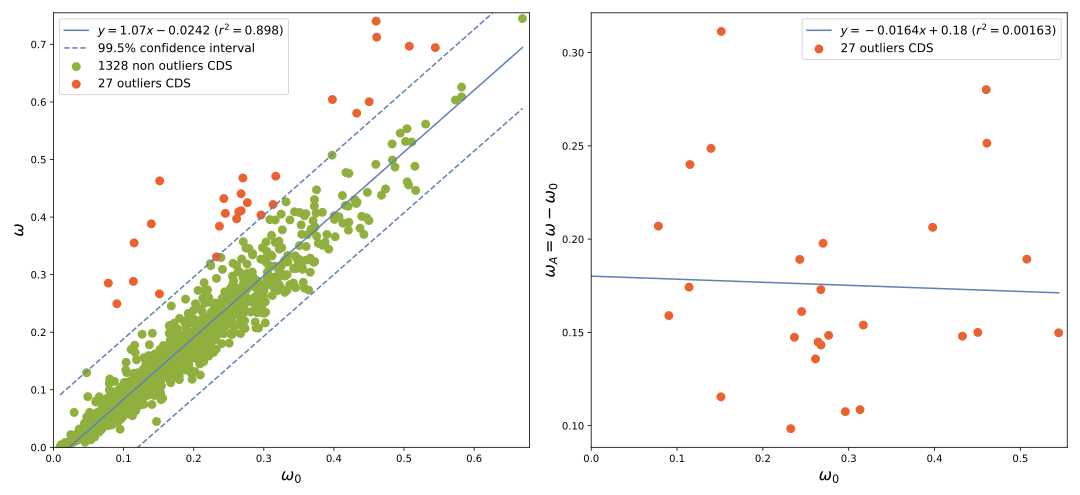
\includegraphics[width=\textwidth]{../Figures/figure_1.pdf}\\
		\caption{ \textbf{Detection of protein-coding sequences ongoing adaptation}. Left panel: scatter plot of 1355 protein-coding sequences, estimation of $\omega$ (y-axis) by the site-model on PhyloBayesMPI and $\omega_{0}$ (x-axis) by the mutation-selection site-model on PhyloBayesMPI. The linear correlation shows a good empirical fit but outliers (in red) are CDS with significantly high $\omega_A = \omega - \omega_{0}$. Right panel: scatter plot of 27 outliers CDS, estimation of $\omega_A$ (y-axis) and $\omega_{0}$ (x-axis). The linear correlation is very poor suggesting that $\omega_A$ effectively extract the adaption regardless of the background of purifying selection ($\omega_0$)  \label{fig:omega_pb}}
	\end{mdframed}
\end{figure*}

	Polymorphism in \textit{Homo sapiens} was downloaded from \href{http://www.ensembl.org/index.html}{ensembl.org}, we used the GRCh38 assembly and mutations from the phase 3 of the 1000 genomes projects \cite{consortium_integrated_2012, the_1000_genomes_project_consortium_global_2015}. Mutations not in inside CDS we discarded at the beginning of the analysis. Insertion and deletion were not analyzed, and only Single Nucleotide Polymorphism (SNPs) with only one mutant allele were kept. Stop codon as the mutant allele were also discarded. Divergence data between \textit{Homo sapiens} and \textit{Pan troglodytes} were extracted from \href{http://www.orthomam.univ-montp2.fr}{OrthoMaM} database \cite{ranwez_orthomam:_2007, douzery_orthomam_2014}. The pipeline (figure \ref{fig:pipeline}) for assembling and analyzing the data is written in python 3.5, the code under GNU license and available at \href{https://github.com/ThibaultLatrille/AdaptaPop}{https://github.com/ThibaultLatrille/AdaptaPop}. \\
	
	One proposed correction for slightly deleterious polymorphism is to drop “rare” polymorphisms, but this method has no clear cut. Dropping singletons provides a simple correction \cite{templeton_contingency_1996}, while other authors (Fay et al. 2002, Smith and Eyre-Walker 2002, Gojobori et al. 2007) have suggested only including polymorphisms with minor allele frequencies above $10\%$ \cite{smith_adaptive_2002, fay_testing_2002, gojobori_adaptive_2007}. We applied this correction to compute $\omega_A^{MK}$. On the contrary, the method of Galtier to compute $\omega_A^{DFEM}$ allow us to keep all polymorphisms, but since the folded site-frequency spectra (SFS) had $2504$ categories (The 1000G project sequenced 2504 diploid individuals) the model was then over-parametrized, and we sub-sampled the folded SFS down to 12 categories using hyper-geometric distribution (sampling without replacement). The effect of sub-sampling is shown in figure \ref{fig:omega_snp}, panel B.
	

	\section*{Results}
	\begin{figure*}[hbt!]
		\begin{mdframed}
			\centering
			\includegraphics[width=\textwidth]{../Figures/figure_3.pdf}\\
			\caption{ \textbf{Empirical distribution of $\omega_A^{MK}$}
				We computed $\omega_A^{MK}$ on the concatenate of the $27$ CDS having a high rate of adaptation, detected in phylogeny-based inference. We compared the result to the empirical distribution of $\omega_A^{MK}$ in the set of all CDS by sampling $27$ random CDS from the $1453$ CDS $1000000$ times (panel A).
				We observed a $p_{\mathrm{value}}=0.119$, meaning that focusing the group of CDS evolving faster than expected in mammals, the rate of adaption measured in population-based inference, in \textit{Homo sapiens} and \textit{Pan troglodytes} is not significantly different from a random sample of sequences.
				Using the site-frequency spectra of SNPs, we computed $\omega_A^{DFEM}$ in the same set of outliers by concatenating the $27$ site-frequency-spectrum (panel C). We compared the result to the empirical distribution of $\omega_A^{DFEM}$ in the set of all CDS by sampling $27$ random CDS from the $1453$ CDS $10000$ times (panel D). Modeling change in population size and the distribution of fitness effects of mutations using the GammaExpo model was not sufficient to observe a significant difference between outliers and the the set of all CDS ($p_{\mathrm{value}}=0.058$). \label{fig:omega_snp}}
		\end{mdframed}
	\end{figure*}
	
	\subsection*{Detecting protein-coding sequences under adaptation}
	$\omega$ estimated by the site-model and $\omega_{0}$ estimated by the mutation-selection site-model shows a good linear correlation ($r^2=0.898$) meaning the mutation-selection site-model effectively predict the rate of non-synonymous substitutions over the rate synonymous substitutions. The assumption that fitness profile of amino-acids are stable in time seems not to be broken (see figure \ref{fig:omega_pb}, left panel).
	Also, for each value of $\omega_{0}$ we computed the $99.5\%$ confidence interval around the predicted value $\omega$.  We detected $27$ CDS (protein coding sequences) having a value of $\omega$ above the upper bound of the confidence interval, meaning the value of their $\omega$ is too high regarding to their $\omega_{0}$. In such outliers, the assumption that fitness landscape are stable in time is broken, and these CDS are considered under adaptive process.  
	To note, we detected no CDS with $\omega$ below the lower bound of the confidence interval. 
	In the outliers, we computed  $\omega_A = \omega - \omega_0$, and asserted that $\omega_A$ correlates poorly with $ \omega_0$ ($r^2=0.002$), suggesting that $\omega_A$ effectively extract the adaption regardless of the background of purifying selection (see figure \ref{fig:omega_pb}). \\
	
	
	On the set of outliers, we performed Fisher's exact to estimates ontology enrichment by contrasting with the set of all CDS (see figure \ref{fig:ontology}). We observed $10$ ontologies with an $e_{\mathrm{value}} <1$, while in expectation we should have observed only $1$ ontology if they were assigned randomly, and the false discovery rate is $10 \%$. In these $10$ ontologies, $60 \%$ were related to immune process, which is similar to results found in large scale analysis (16,529 CDS, Kosiol \textit{et al} \cite{kosiol_patterns_2008}). We conclude that our method for detecting adaptation effectively extract adaptation regardless of the background of purifying selection, and extracted primarily sequences related to immune process. \\
	
			\end{multicols}
\begin{table}[ht!]
\centering
\begin{adjustbox}{width = 1\textwidth}
	\small\begin{tabular}{|c|c|c|c|c|c|}
		\hline
		Ontology & $n_{\mathrm{Observed}}$ & $n_{\mathrm{Expected}}$ & Odds ratio & $p_{\mathrm{value}}$ & $e_{\mathrm{value}}$\\
		\hline
		plasma membrane & $12$ & $3.48$ & $3.45$ & $0.00232$ & $0.195$\\
		protein heterodimerization activity & $4$ & $0.459$ & $8.71$ & $0.00241$ & $0.202$\\
		regulation of immune response & $2$ & $0.0566$ & $35.3$ & $0.00369$ & $0.31$\\
		T cell differentiation & $2$ & $0.0755$ & $26.5$ & $0.00546$ & $0.459$\\
		immune system process & $6$ & $1.36$ & $4.4$ & $0.00584$ & $0.49$\\
		response to stress & $8$ & $2.24$ & $3.57$ & $0.00608$ & $0.511$\\
		innate immune response & $4$ & $0.659$ & $6.07$ & $0.00765$ & $0.643$\\
		receptor activity & $3$ & $0.348$ & $8.61$ & $0.00845$ & $0.71$\\
		metabolic process & $6$ & $1.51$ & $3.98$ & $0.00899$ & $0.755$\\
		leukocyte migration & $2$ & $0.113$ & $17.6$ & $0.00995$ & $0.836$\\
		\hline
	\end{tabular}
\end{adjustbox}
\caption{\textbf{Ontology enrichment in the outliers}. 84 Fisher's exact test performed with 27 CDS detected as adaptive and 1328 as non-adaptive. In the table is solely shown the tests with an  $e_{\mathrm{value}}$ lower than $1$. In terms of false positive discovery rate, it means that on the $10$ ontologies observed we expected $1$ on average, and the posteriori rate of false discoveries is $10\%$.  \label{fig:ontology}}
\end{table}
\begin{multicols}{2}
	
	We also tried the one step procedure to estimate $\omega_A^*$ but it was not conclusive since $\omega^*$ captured also part the purifying process, and thus it was not not possible to untie the purifying process from adaptation. 
	

	\subsection*{Congruence between phylogeny- and population-based inference}
	We computed $\omega_A^{MK}$ on the concatenate of the $27$ CDS having a high rate of adaptation, detected in phylogeny-based inference. We compared the result to the empirical distribution of $\omega_A^{MK}$ in the set of all CDS by sampling $27$ random CDS from the $1453$ CDS $1000000$ times (see figure \ref{fig:omega_snp}, panel A).
	We observed a $p_{\mathrm{value}}=0.119$, meaning that focusing the group of CDS evolving faster than expected in mammals, the rate of adaption measured in population-based inference, in \textit{Homo sapiens} and \textit{Pan troglodytes} is not significantly different from a random sample of sequences.
	
	Using the site-frequency spectra of SNPs, we computed $\omega_A^{DFEM}$ in the same set of outliers by concatenating the $27$ site-frequency-spectrum (see figure \ref{fig:omega_snp}, panel C). We compared the result to the empirical distribution of $\omega_A^{DFEM}$ in the set of all CDS by sampling $27$ random CDS from the $1453$ CDS $10000$ times (see figure \ref{fig:omega_snp}, panel D). Modeling change in population size and the distribution of fitness effects of mutations using the GammaExpo model was not sufficient to observe a significant difference between outliers and the the set of all CDS ($p_{\mathrm{value}}=0.058$).
	
	\section*{Discussion}
	Using phylogeny-based inference, we can discover protein coding sequences (CDS) under adaptation when the $\omega$ estimated by the site-model deviates significantly from the mutation-selection null model ($\omega_0$). We observed $27$ CDS from $1355$ ($2\%$) as outliers, and they showed significant increase in ontology related to immune process. Moreover the deviation from quasi-neutrality is not depend of the strength of the purifying process. At the level of a CDS, we can tease out adaptation and purifying selection with the help of mutation-selection models. Theoretically, the rate of adaptation can be estimated in one run ($\omega_A^*$), but it the computation was not stable.\\
	
	A first limitation of the results is that we restricted our analysis to $1355$ CDS because of time and computation constrains. However we can run the procedure on the whole dataset of $11256$ CDS to give more statistical power to the results. Phylogeny-based inference is computationally intensive, and require a well resolved species tree, hence our limitations to mammals. Moreover it crucially depends on the quality of the alignments, and paralogs identified as orthologs can easily falsify the results. Practically, we could also extend our analysis by using population data widely available for the mouse instead of restricting to \textit{Homo sapiens}. More broadly, we can extend our analysis to numerous clades where both population and phylogenetic data are widely available, such as drosophila. \\
	
	On the other hand, population-based inference is more coarse grained and the polymorphism available for each CDS is not enough to estimate $\omega_A$ reliably for each sequence and one need to concatenate sequences. The set of CDS having a high rate of adaptive evolution detected by phylogeny-based inference did not show a significant increase in the rate of adaptation inferred by population-based method. This result raise biological questions and methodological issues. If we assume that both methods are performing well to detect adaptation, this result means that the CDS evolving fast in mammals are not necessarily the sequences evolving fast in the \textit{Hominini}. In the other hand, this result could be a methodological issue, meaning phylogeny- and population-based inference are inherently testing for different adaptive rate, and that they should have no theoretical reason to be the same. Indeed if sequences are evolving very rapidly, sequences will not aligned and be discarded by the analysis altogether and not detected (false negative). On the other hand, population-based inference can not detect long term changes of the evolutionary process. Especially since the purifying process is stronger on longer timescale, the frontier between neutral and mildly deleterious mutation is blurred on short timescale. 
	
	Altogether, this preliminary study suggest that the integration between population and phylogeny-based inference raises theoretical and practical issues. We suggest that further investigating these methodological integration will provide biological insight on the evolutionary constrain of protein-coding sequences. \\
	
	\section*{Author contributions and acknowledgments}
	I thank Nicolas Lartillot for his help, support and advises all along the internship and concerning this report, as well as for insightful discussions. I thank the team for the great atmosphere at the lab, and Fidel Botero-Castro for providing cleaned mammalian alignment data. The personal equipment was provided by ANR Dasire. This work was performed using the computing  facilities of the CC LBBE/PRABI. I wrote all the python code of the pipeline \ref{fig:pipeline}, and I designed the statistical tests and analyze the data. The repository for the pipeline and this report is available at \href{https://github.com/ThibaultLatrille/AdaptaPop}{https://github.com/ThibaultLatrille/AdaptaPop}.

	\bibliographystyle{unsrt}
	\bibliography{codon_models,adaptapop}
	
	\end{multicols}
\end{document}
